% ********************************************
%
%   Dear Authors,
% 
%   Please, read the following comments in Preset settings and adjust the settings according to your needs.
%   Please, feel free to add more packages or macros if needed.
%   Details of the pre-defined packages, symbols and macros can be found in the submodule "template". (See PDF files.)
%   If you finished the adjustments, you can remove the comments for a clean document.
% 
%   Any questions or contributions are welcome.
%   Please, contact to the author.
%   Enjoy your writing.
%
%                               Myeongseok Ryu
%  	    				dding_98@gm.gist.ac.kr
%                                  09.Feb.2025
%
% ********************************************

% ********************************************
% Revision History
%   - 01.Jun.2025: Conference template created.
% ********************************************

% ********************************************
% This project is highly ispired by the work of LMRES Lab, Hochschule München.
% Thank you very much my dear friend, Niklas Monzen, for your kind support.
% ********************************************

% ============================================
%         Preset 1. Document Type
% ============================================
\documentclass[conference]{IEEEtran}

% THIS IS NEEDED FOR FINAL SUBMISSION
\IEEEoverridecommandlockouts 
% This command is only needed if you want to use the \thanks commands  
%\overrideIEEEmargins 
% Needed to meet printer requirements.

% ============================================
%         Preset 2. Local Path
% ============================================
% When you create "figures" or "movies" directories in the "src" (source code) directory, the file name including path can be long.
% To avoid this, and to make it easier to adjust, you can define the alias for the path.
% The examples are provided below.

\newcommand*{\FIGURESPATH}{./figures}
% \newcommand*{\SIMFIGURESPATH}{./src/script_simulation/figures}
% \newcommand*{\SLXFIGURESPATH}{./src/simulink_simulation/figures}
% \newcommand*{\MOVIESPATH}{./movies}

% ============================================
%         Preset 3. Pre-defined Settings
% ============================================
% PLEASE DO NOT ADD OR REMOVE PACKAGES IN THE SUBMODULE LOCALLY!
% CONTACT THE AUTHOR FOR ADJUSTMENTS.
%
% The packages are pre-defined in the submodule "Template".
% If you need more packages, please add them after using pre-defined packages.

\def\pub{false} % true for publication, false for draft
\newcommand*{\template}{template} 
\input{\template/preamble/preamble_conf.tex}

% ============================================
%     Preset 4. Additional Corrections
% ============================================
% correct bad hyphenation here
% \hyphenation{op-tical net-works semi-conduc-tor}
% \pagestyle{empty}

\begin{document}

% ============================================
%            TITLE and AUTHORS
% ============================================
\title{
  Example Title of Conference
  % {\footnotesize \textsuperscript{*}Note: Sub-titles are not captured for       https://ieeexplore.ieee.org  and
  % should not be used}
  \thanks{
      This work was supported by my 10 fingers and Macbook Air M1.
  }
} 

\author{
    \IEEEauthorblockN{1\textsuperscript{st} Myeongseok Ryu}
    \IEEEauthorblockA{\textit{Cho Chun Shik Graduate School of Mobility} \\
    \textit{Korean Advanced Institute of Science and Technology (KAIST)}\\
    Daejeon, Republic of Korea \\
    dding\_98@kaist.ac.kr}
\and
    \IEEEauthorblockN{2\textsuperscript{nd} Niklas Monzen}
    \IEEEauthorblockA{\textit{Laboratory for Mechatronic and Renewable Energy Systems} \\
    \textit{Hochschule München (HM) University of Applied Sciences}\\
    Munich, Germany \\
    niklas.monzen@hm.edu}
}

\maketitle 
\thispagestyle{empty}

% ============================================
%         ABSTRACT and KEYWORDS
% ============================================
\begin{abstract}
  Hallo, this is an example of an abstract.
  \lipsum[1]
\end{abstract}

\begin{IEEEkeywords}
    Example, IEEEtran, journal, \LaTeX, template.
\end{IEEEkeywords}

% ============================================
%         Notation
% ============================================
\section*{Notation}
In this study, the following notation is used:

\begin{itemize}
    \item $\R^n$ denotes the $n$-dimensional Euclidean space.
    \item $\R^{n\times m}$ denotes the set of $n\times m$ real matrices.
    \item $\otimes$ denotes the Kronecker product \cite[Chap. 7 Def. 7.1.2]{Bernstein:2009aa}.
    \item A vector and a matrix are denoted by $\mv{x}=[x_i]_{i\in\{1,\cdots,n\}}\in\R^n$ and $
        \mm A
        := 
        [a_{ij}]
        _{
            i\in\{1,\cdots,n\},j\in\{1,\cdots ,m\}
        }\allowbreak\in\R^{n\times m}
        $, respectively.
    \item $\myrow_i(\mm A)$ denotes the $i\textsuperscript{th}$ row of the matrix $\mm A\in\R^{n\times m}$. 
    \item For $\mm{A}\in\R^{n\times m}$, denotes the vectorization of $\mm A$, $\myvec(\mm A):=(\myrow_1(\mm A^\top),\cdots,\myrow_m(\mm A^\top)  )^\top\in\R^{nm}$.
    % \item $\mycol_i(A)$ and $\myrow_j(A)$ denote the $i\textsuperscript{th}$ column and $j\textsuperscript{th}$ row of $A\in\R^{n\times m}$, respectively.
    % \item $\myvec(A):= [\mycol_1(A)^\top  ,\cdots,\mycol_m(A)^\top  ]^\top   $ for $A\in\R^{n\times m}$.
    \item $\lambda_{\min}(\mm A)$ denotes the minimum eigenvalue of the matrix $\mm A\in\R^{n\times n}$.
    \item $\mm I_n$ denotes the $n\times n$ identity matrix, and $\mm 0_{n\times m}$ denotes the $n\times m$ zero matrix.
\end{itemize}

% ============================================
%         SECTION: Dummy Section
% ============================================
\section{Dummy Section}

You can cite a reference like this \cite{Ryu:2024aa}.

\lipsum[1-3]

% ============================================
%         SECTION: Tables and Figures
% ============================================
\section{Tables and Figures}

Refer the following table and figures for examples of tables and figures.

\begin{table}[t]
    \renewcommand{\arraystretch}{1.3}
    \caption{Example of table.}
    \centering
    \begin{tabular}{c m{9.5em} c c c }
    % \begin{tabular}{c c c c c}
    \hline
    \textbf{Symbol} & \textbf{Description} & \textbf{Value} \\
    \hline
    \hline 
    $m_1,m_2$ & Mass & 2.465 kg \\
    \hline
    $l_1,l_2$  & Length & 0.2 m \\  
    \hline
    ${l_c}_1,{l_c}_2$ & Center of mass & 0.139 m \\
    \hline
    $I_1,I_2$  & Inertia & 0.069 kgm\textsuperscript{2} \\
    \hline
    \end{tabular}
    \label{table:example}
\end{table}

\begin{figure}[t]
  \centering
    \subfloat[My love Spezi.]{
      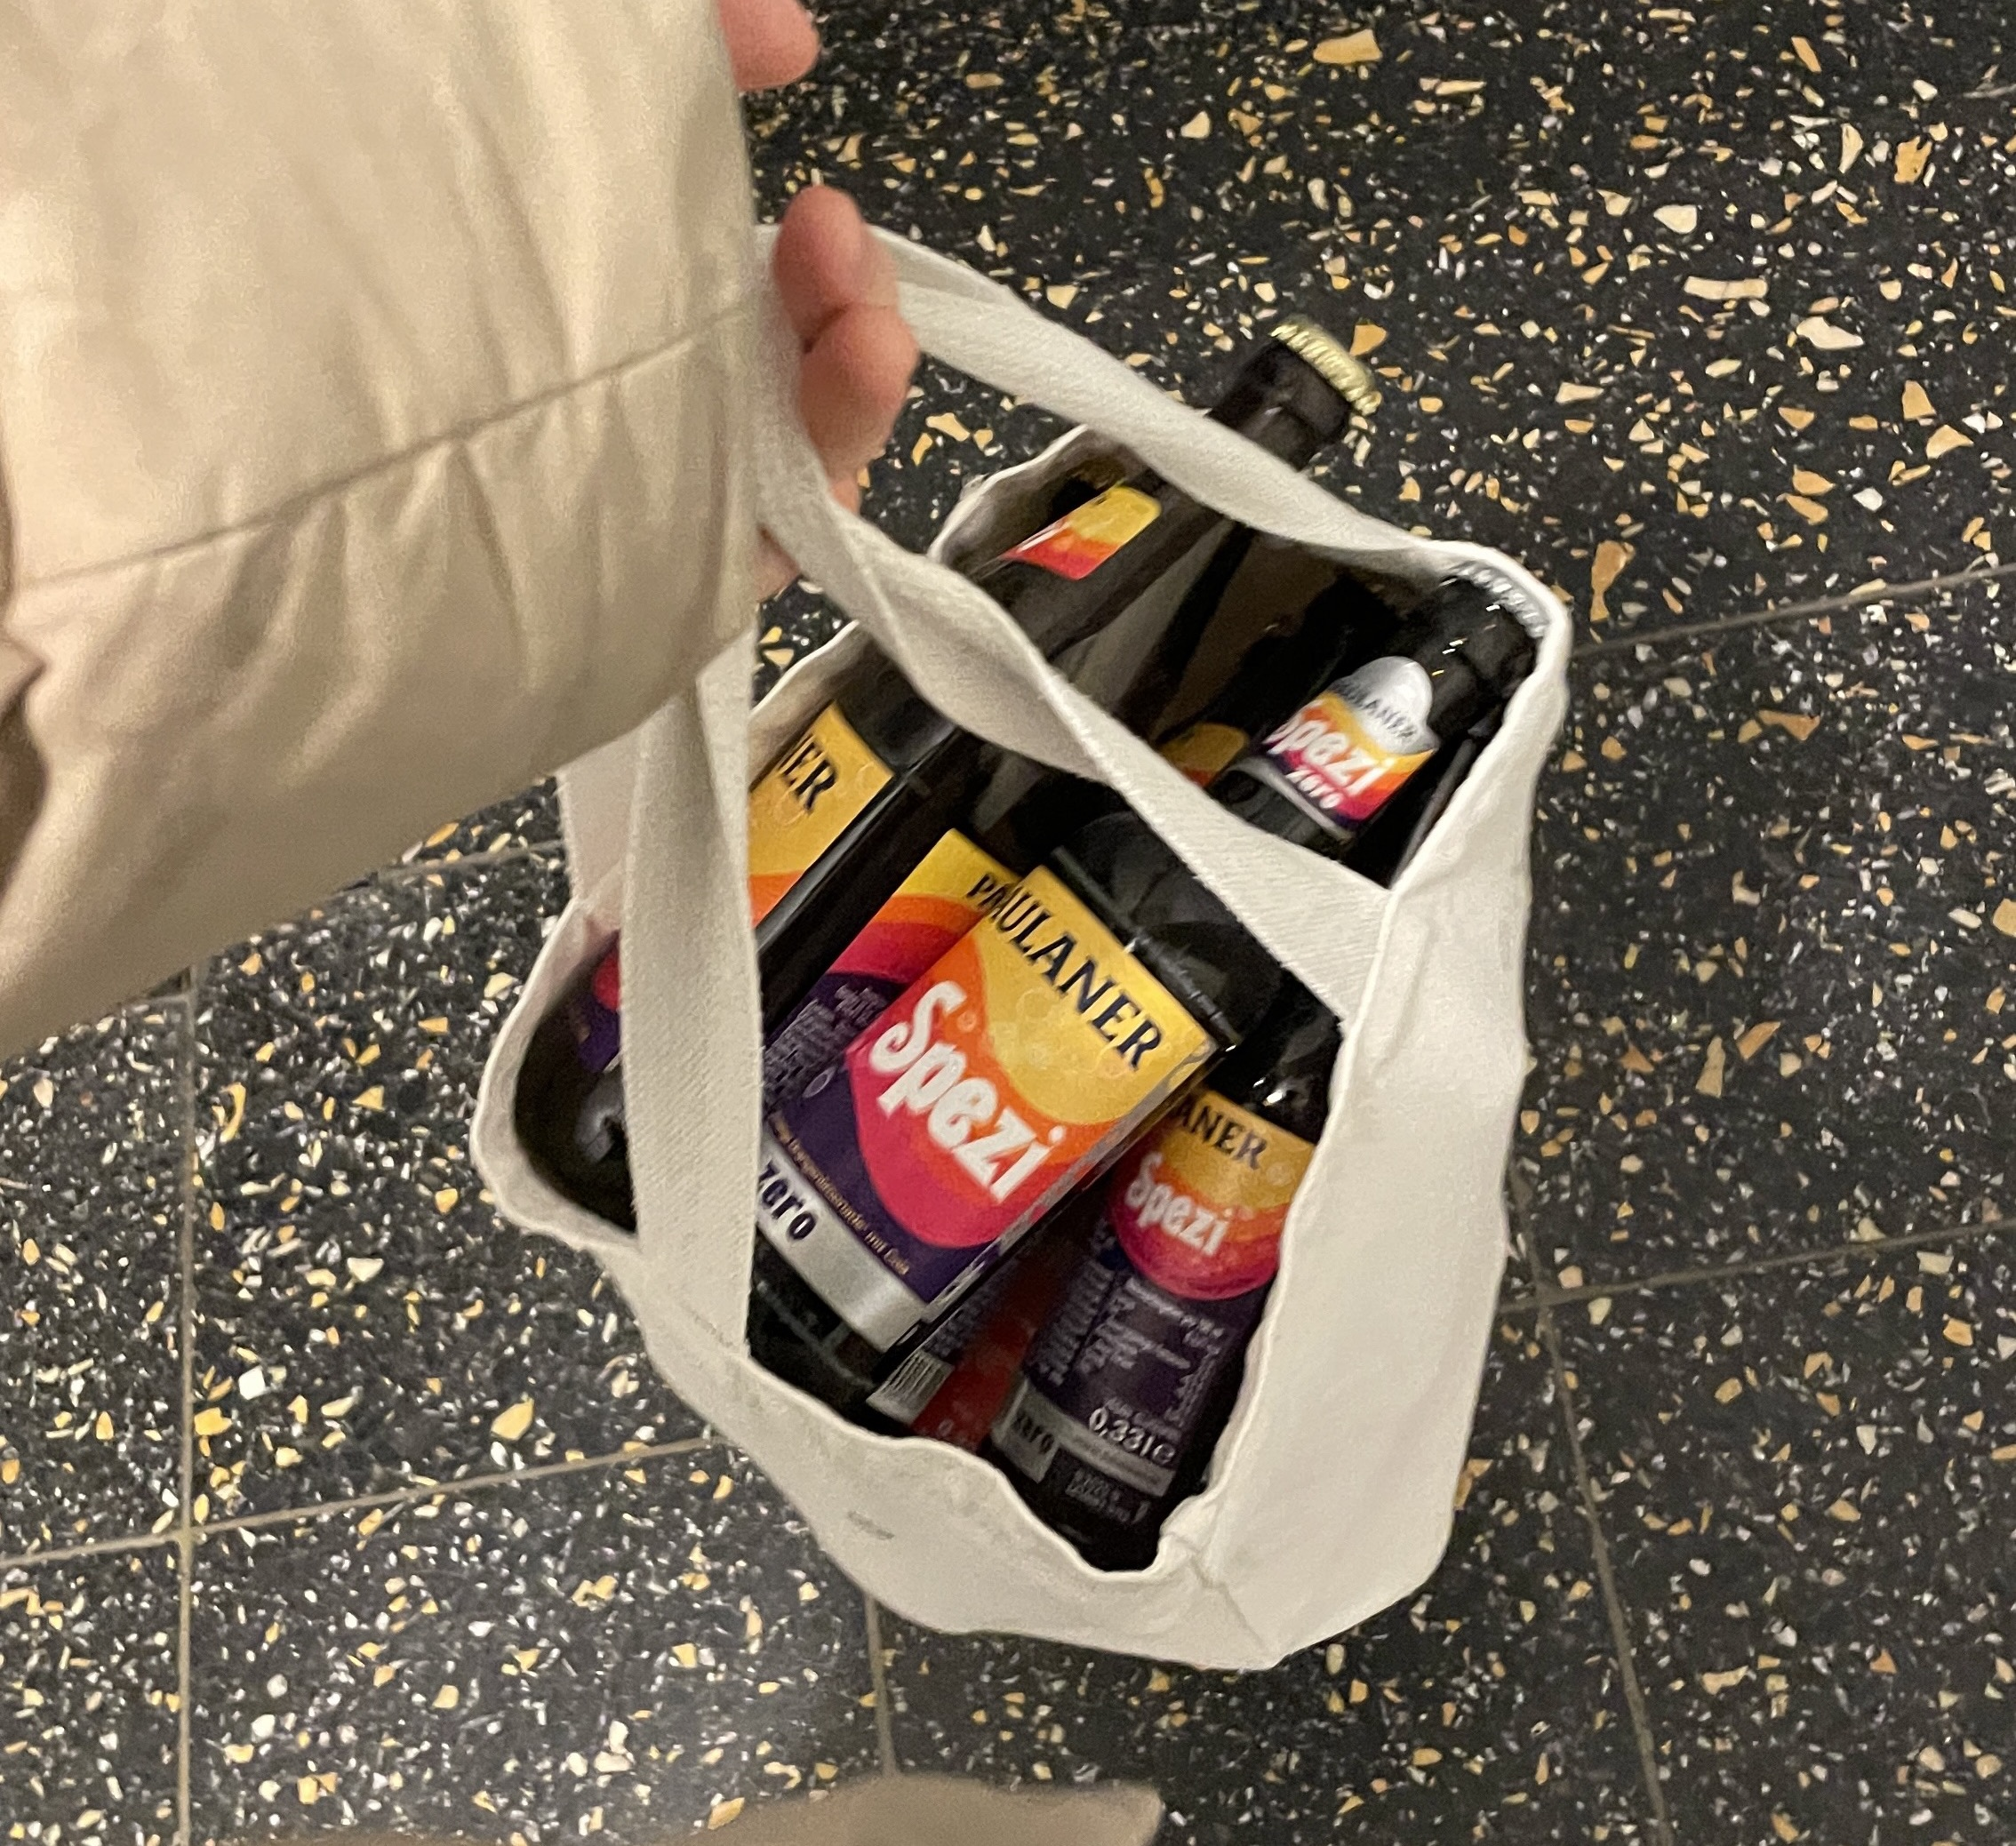
\includegraphics[width=.89\linewidth]
      {
        figures/dummy_figure.JPG
      }%
      \label{fig:example:1}}
    \vfill
    \subfloat[My love Spezi.]{
      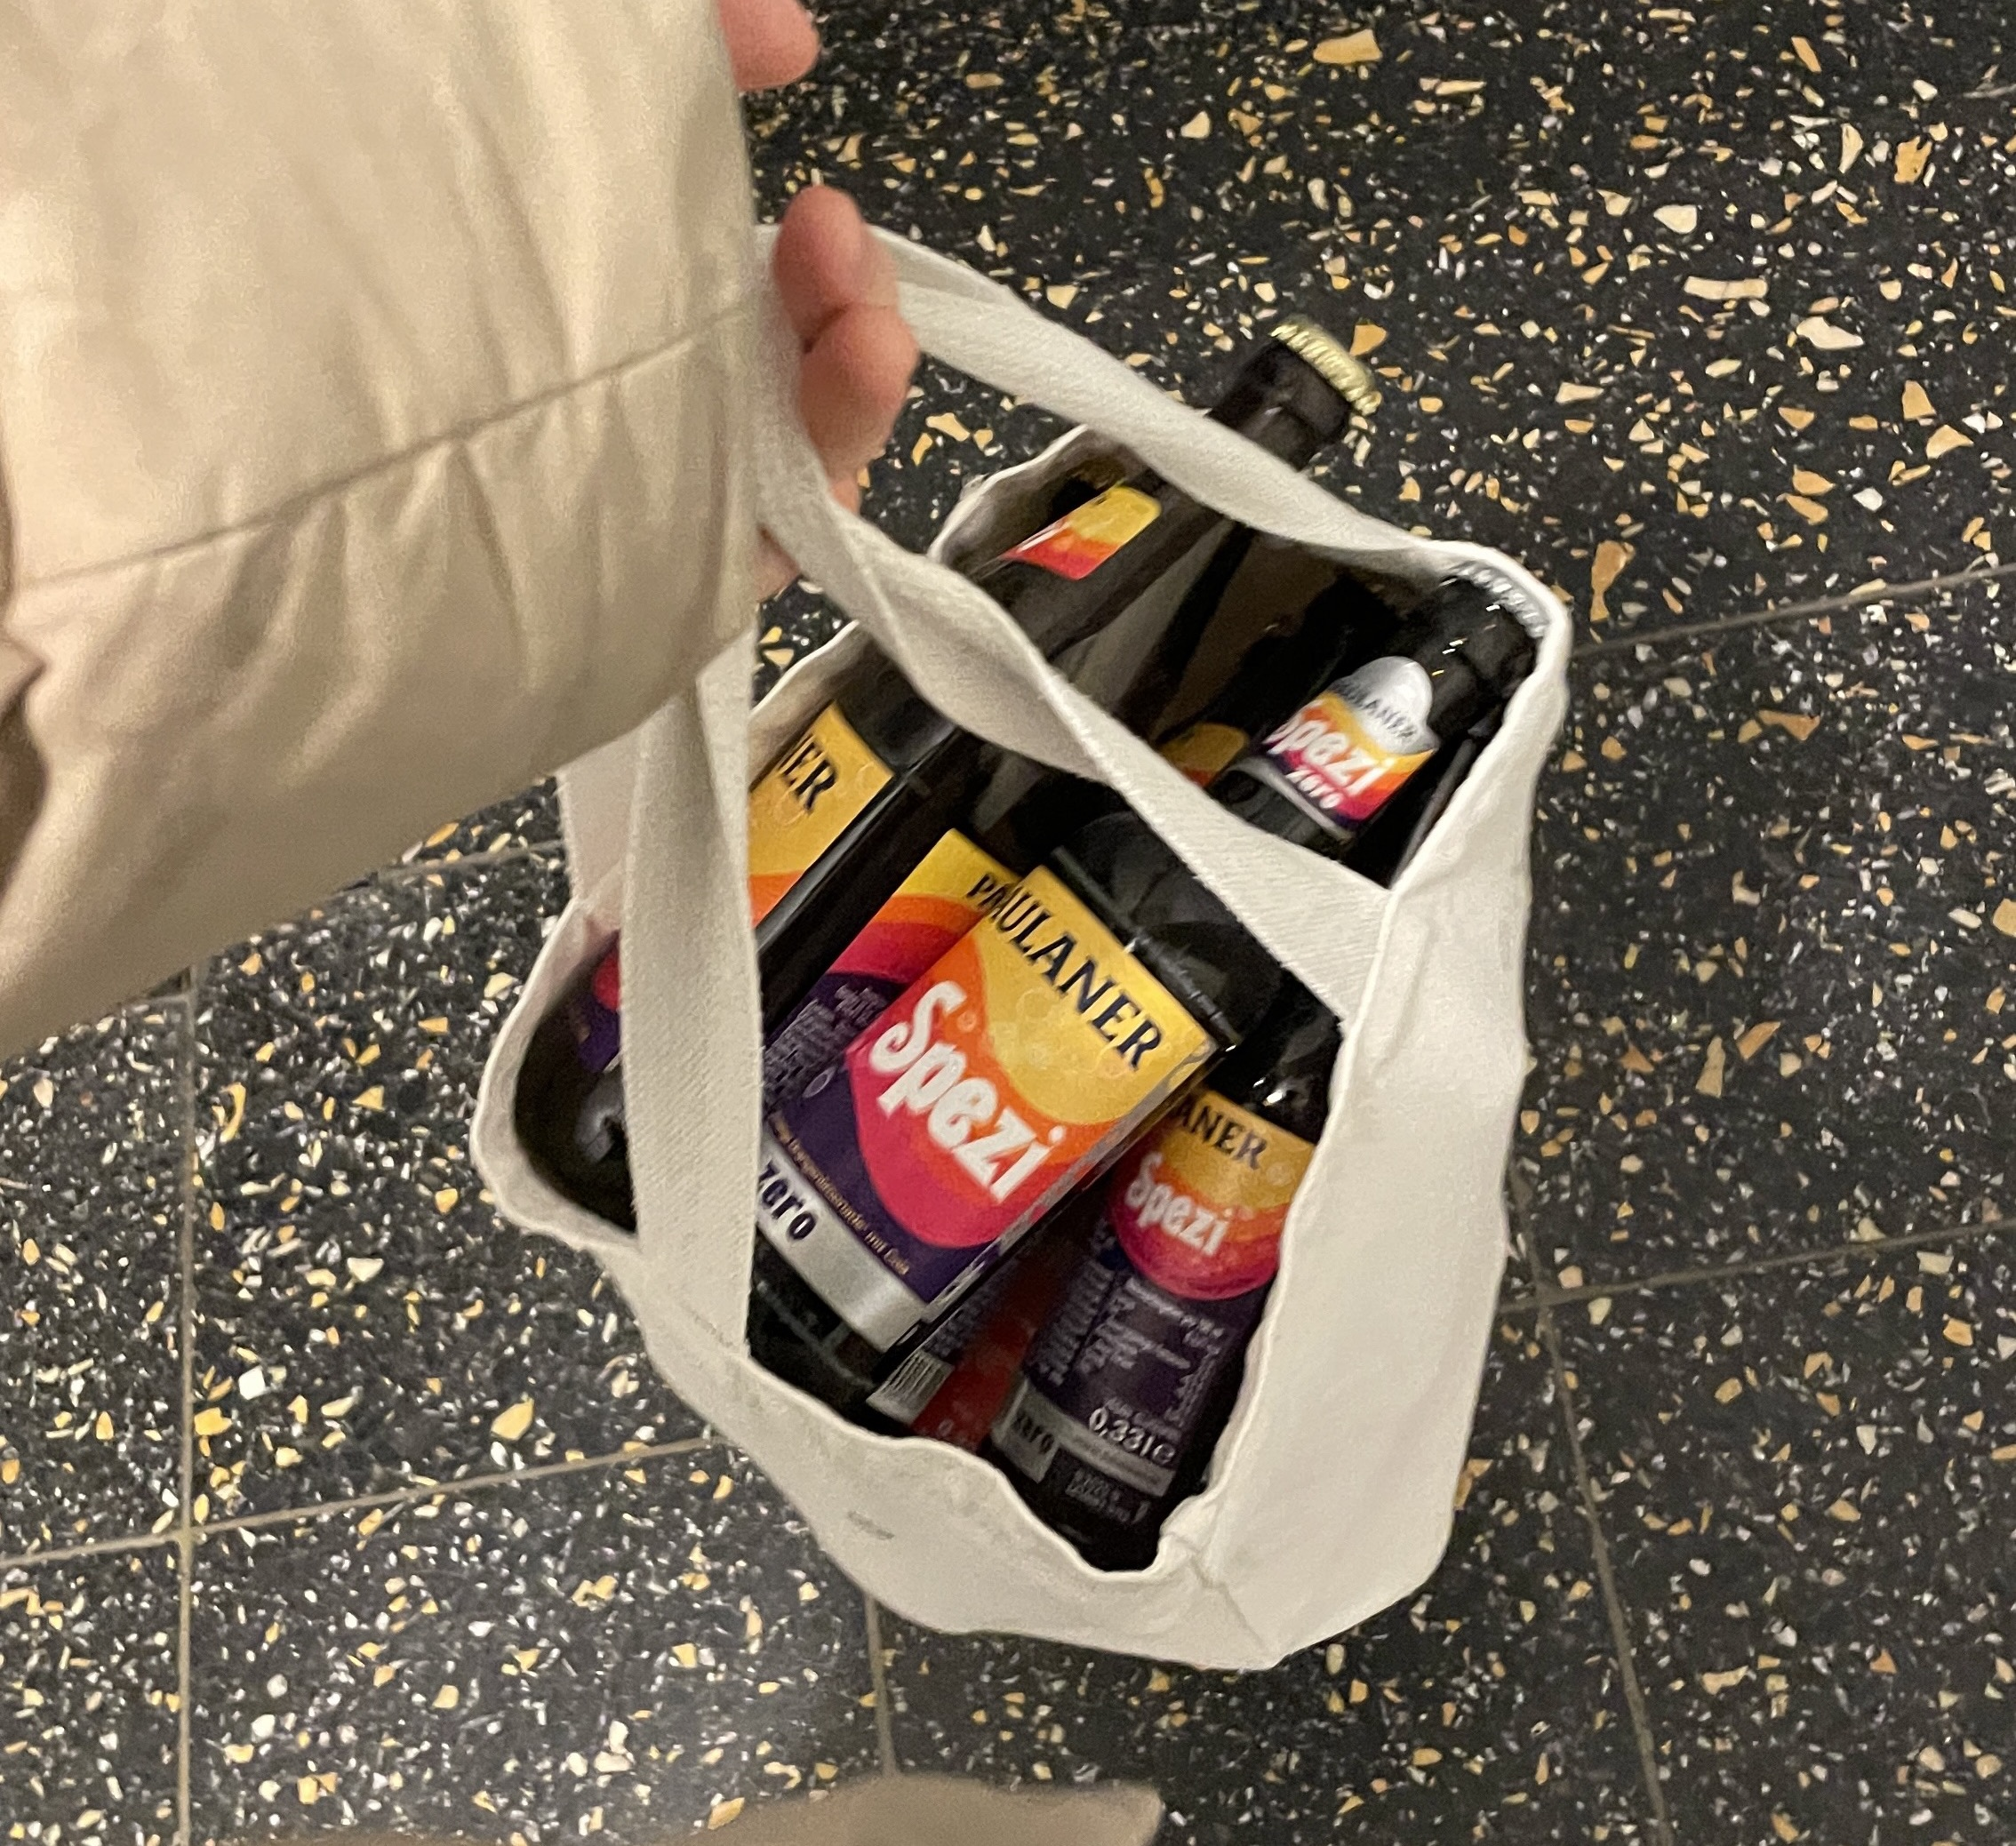
\includegraphics[width=.89\linewidth]
      {
        figures/dummy_figure.JPG
      }%
      \label{fig:example:2}}      
    \caption{
    Example of subfigures.
    You can add colored lines like \protect\colorLine{blue}{solid} or \protect\colorLine{red}{dashed}, \ie you need to use $\protect$ in captions.
    By the way, the drinks in the figures are Spezi, which is my favorite drink in Munich, Germany.
  }
\label{fig:example}
\end{figure}

\begin{figure*}[t]
  \centering
    \subfloat[My love Spezi.]{
      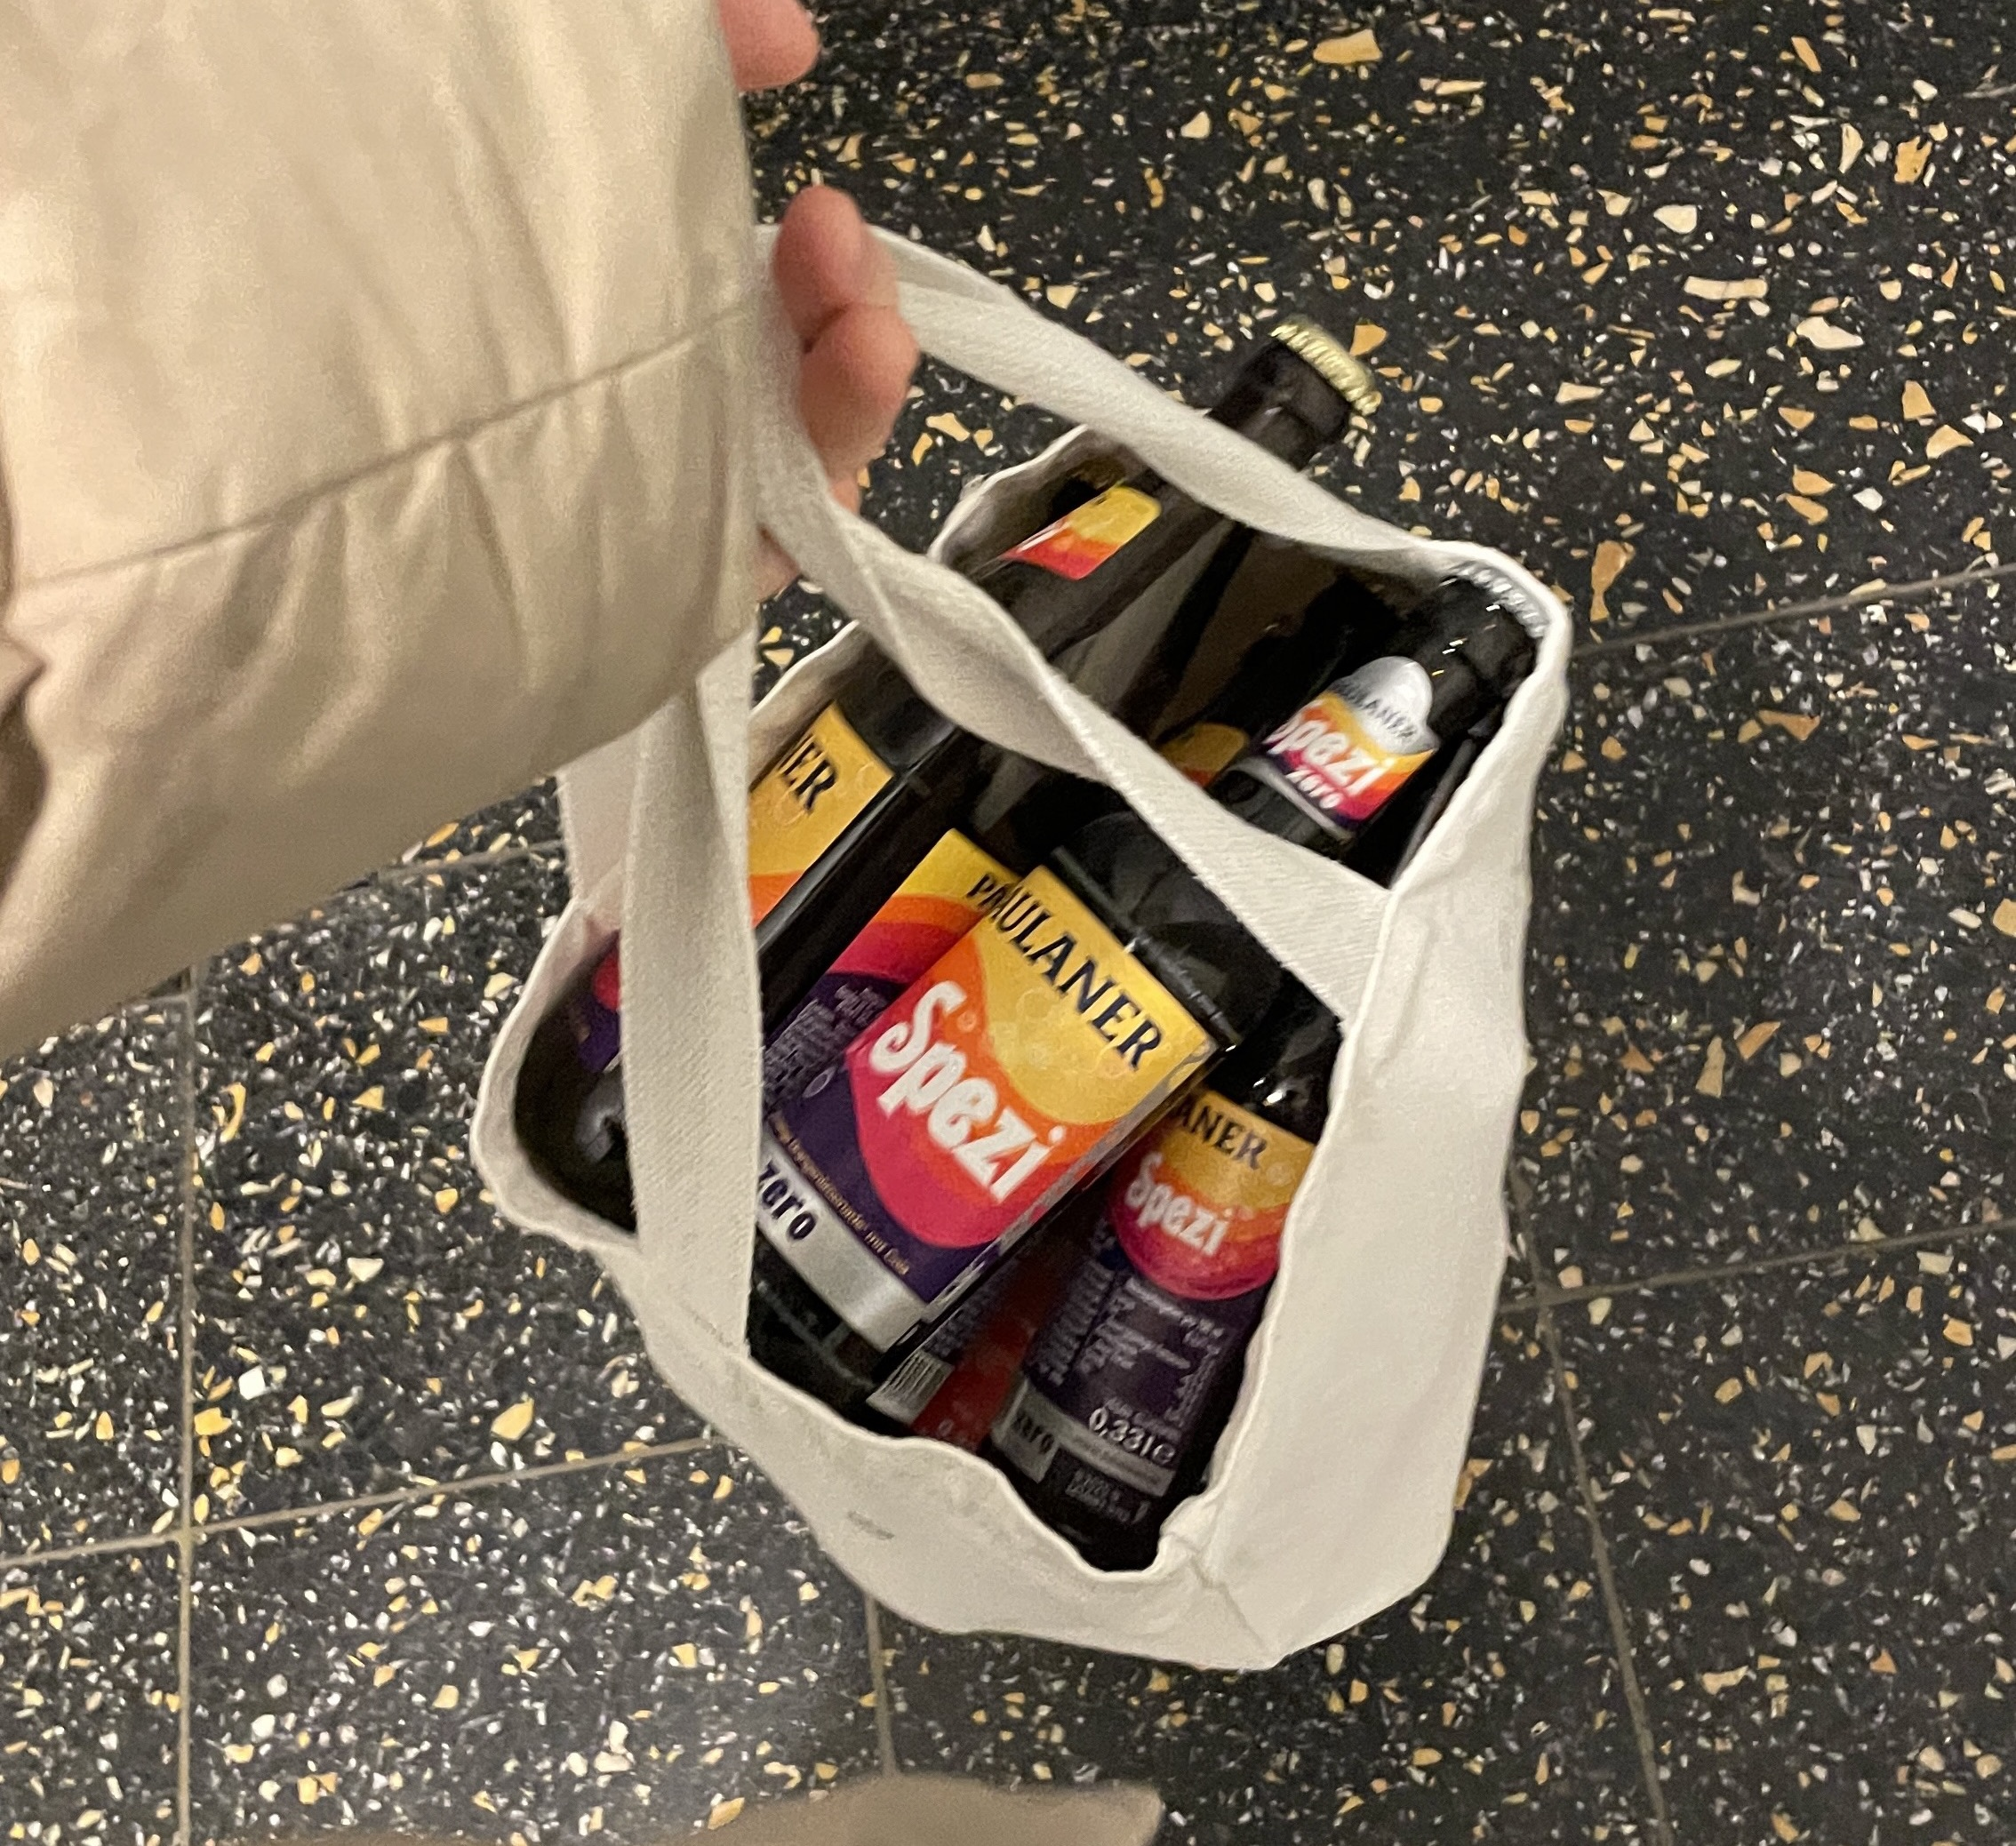
\includegraphics[width=.39\linewidth]
      {
        figures/dummy_figure.JPG
      }%
      \label{fig:example:full:1}}
    \hfill
    \subfloat[My love Spezi.]{
      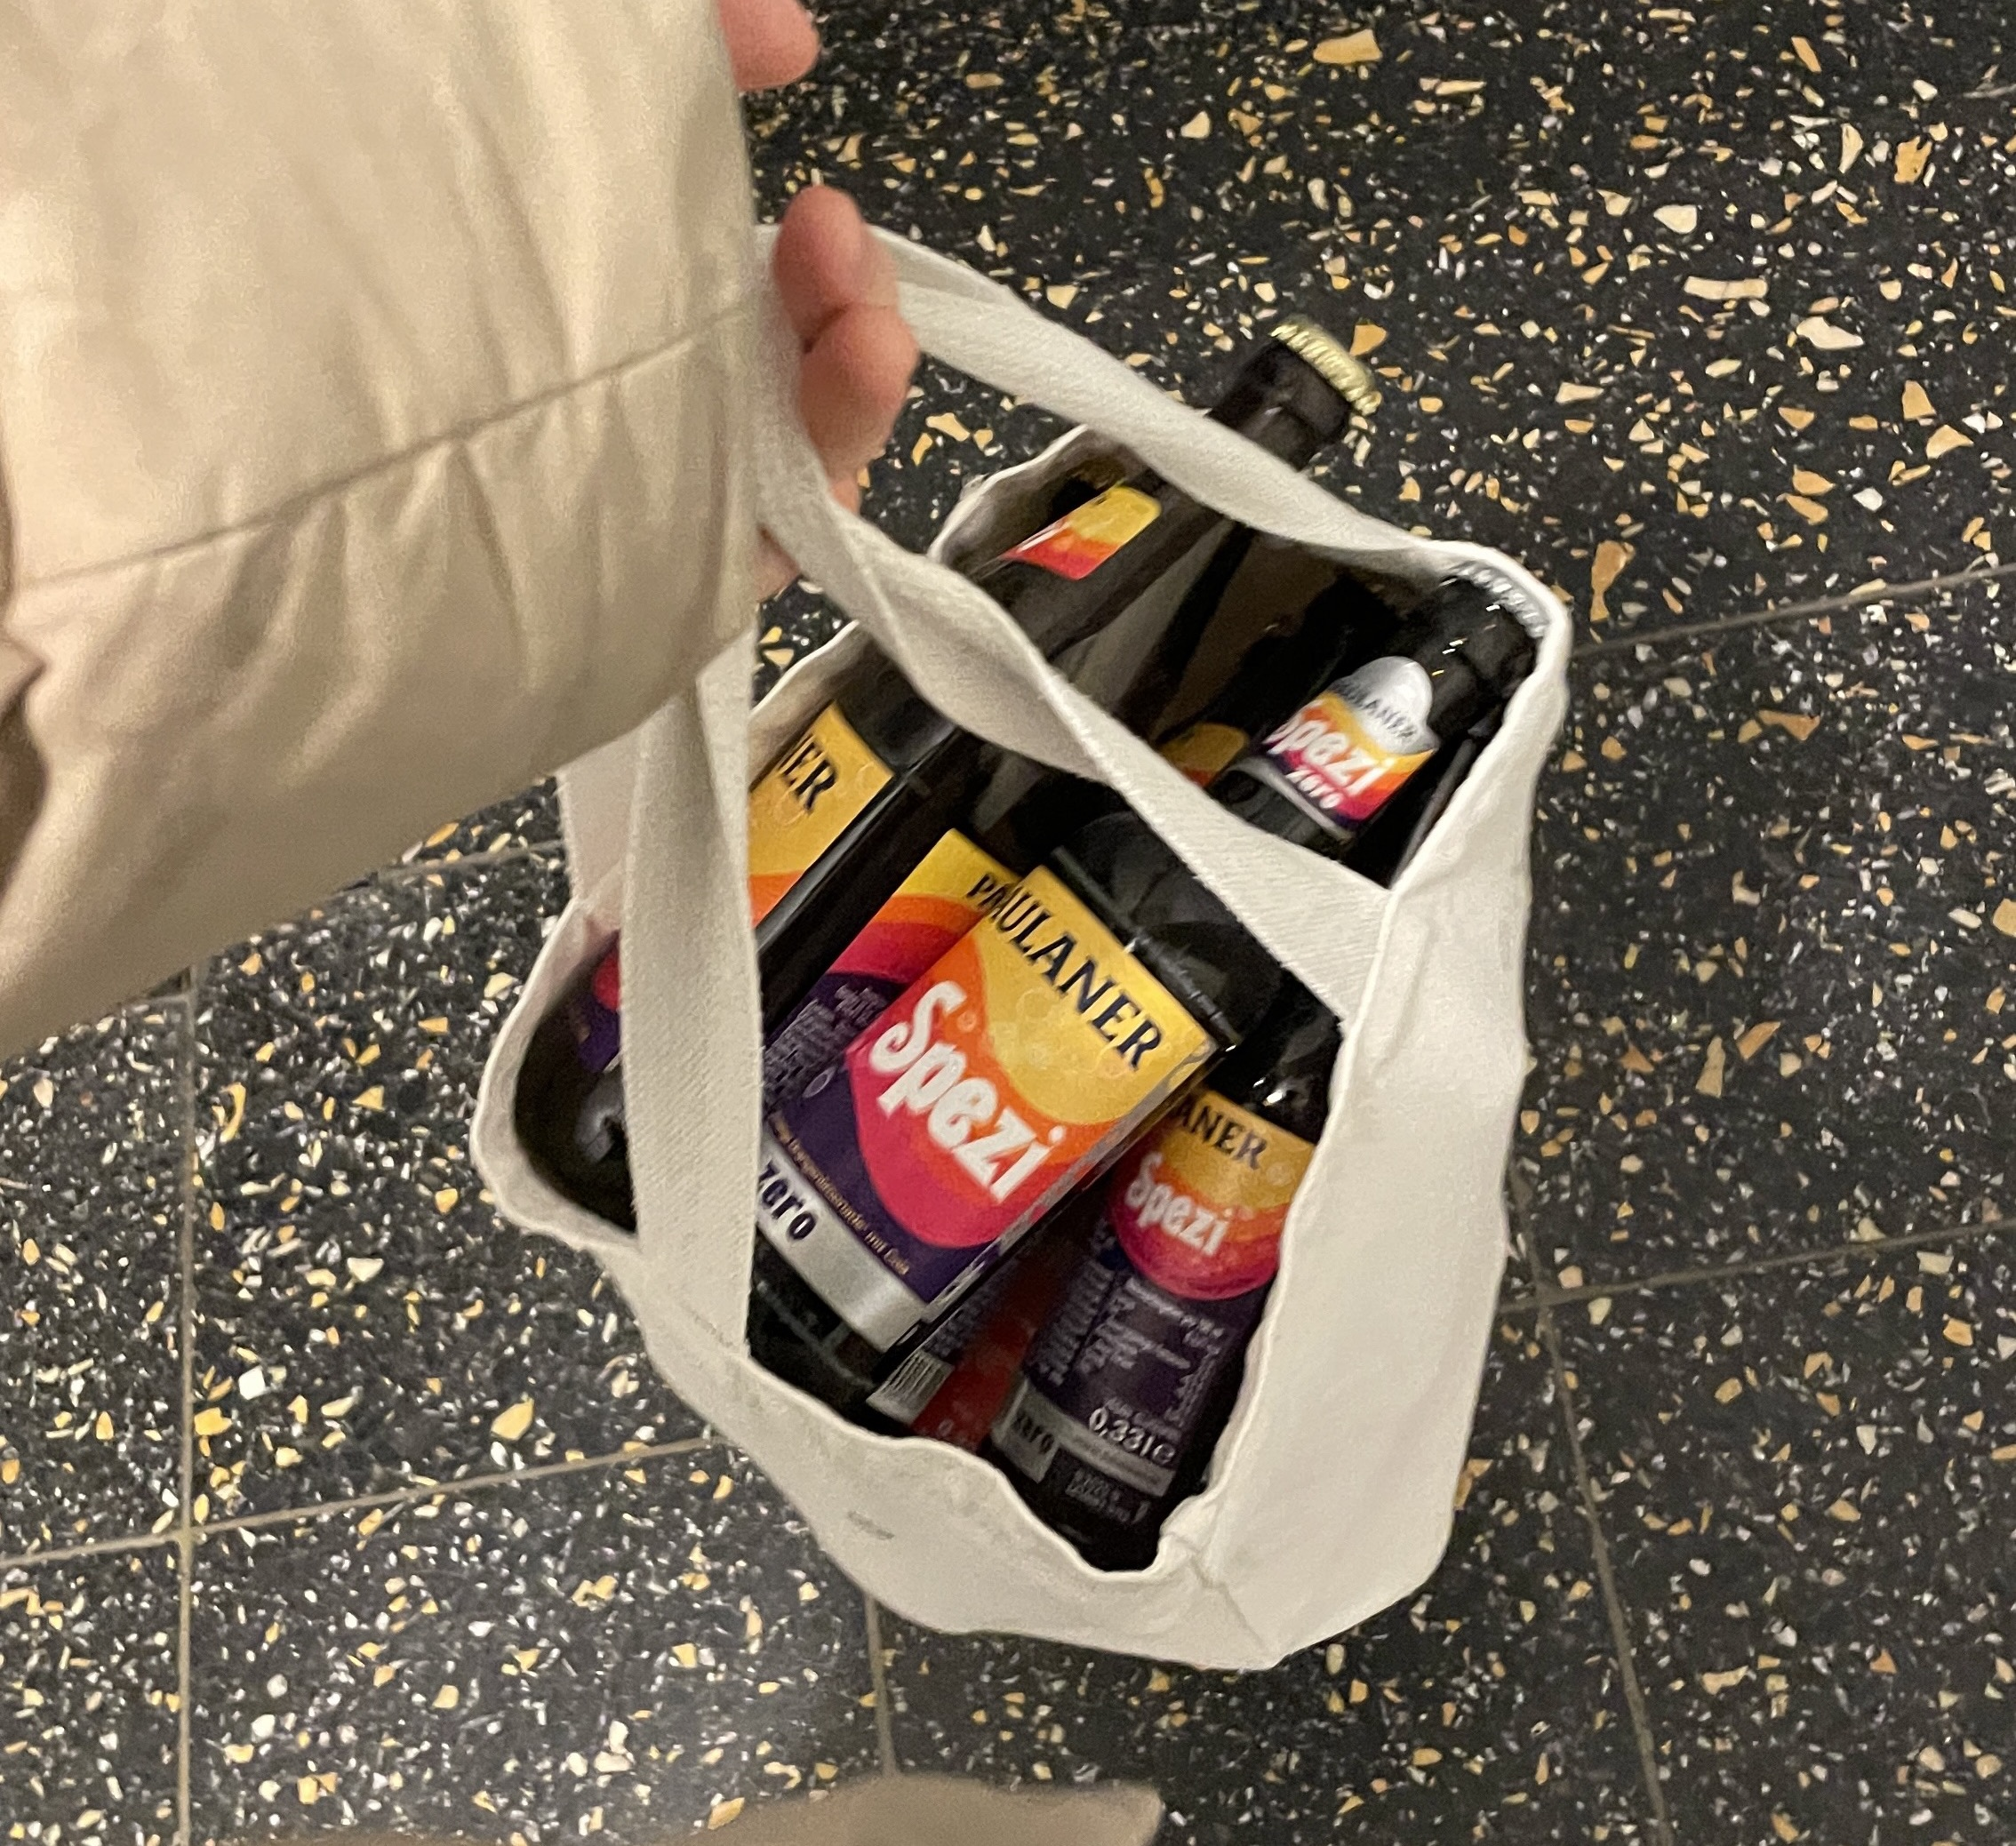
\includegraphics[width=.39\linewidth]
      {
        figures/dummy_figure.JPG
      }%
      \label{fig:example:full:2}}      
    \caption{
    Example of subfigures in full width.
  }
\label{fig:example:full}
\end{figure*}

% ============================================
%                   Appendix
% ============================================
%% The Appendices part is started with the command \appendix;
%% appendix sections are then done as normal sections
\appendix

% ============================================
%                   Bibliography
% ============================================
\bibliographystyle{IEEEtran}
\bibliography{\template/refs}

\end{document}